% XCircuit output "write\_packet.tex" for LaTeX input from write\_packet.eps
\def\putbox#1#2#3#4{\makebox[0in][l]{\makebox[#1][l]{}\raisebox{\baselineskip}[0in][0in]{\raisebox{#2}[0in][0in]{\scalebox{#3}{#4}}}}}
\def\rightbox#1{\makebox[0in][r]{#1}}
\def\centbox#1{\makebox[0in]{#1}}
\def\topbox#1{\raisebox{-0.60\baselineskip}[0in][0in]{#1}}
\def\midbox#1{\raisebox{-0.20\baselineskip}[0in][0in]{#1}}
   \scalebox{1}{
   \normalsize
   \parbox{8.25in}{
   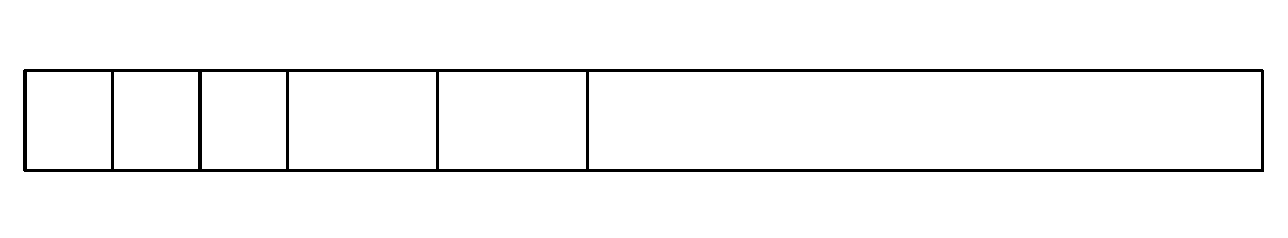
\includegraphics[scale=1]{write_packet.eps}\\
   % translate x=1072 y=150 scale 0.38
   \putbox{8.14in}{1.09in}{1.20}{0}%
   \putbox{0.81in}{1.09in}{1.20}{37}%
   \putbox{1.39in}{1.09in}{1.20}{36}%
   \putbox{1.89in}{1.09in}{1.20}{35}%
   \putbox{2.47in}{1.09in}{1.20}{34}%
   \putbox{2.89in}{1.09in}{1.20}{33}%
   \putbox{3.47in}{1.09in}{1.20}{32}%
   \putbox{3.89in}{1.09in}{1.20}{31}%
   \putbox{5.97in}{0.09in}{1.20}{data}%
   \putbox{0.71in}{-0.2in}{1.20}{\shortstack[lb]{break\\or\\watch}}%
   \putbox{1.37in}{-0.2in}{1.20}{\shortstack[lb]{set\\or\\clear}}%
   \putbox{2.06in}{0.09in}{1.20}{reg\_id}%
   \putbox{2.74in}{0.09in}{1.20}{watch\_reg\_type}%
   \putbox{0.24in}{1.09in}{1.20}{38}%
   \putbox{-0.04in}{0.09in}{1.20}{interrupt}%
   } % close 'parbox'
   } % close 'scalebox'
   \vspace{-\baselineskip} % this is not necessary, but looks better
